\documentclass{article}

\usepackage{graphicx}
\usepackage{amsmath}
\usepackage{algorithm}
\usepackage{algorithmic}
\usepackage[noend]{algpseudocode}


\begin{document}
    \title{Tutorial 2}
    \date{28-07-2019}
    \author{Deepank Agrawal (17CS30011)}
  \maketitle
  
  \section{Problem Statement}
    $P[1..n]$ is an input list of $n$ points on $xy$-plane. Assume that all $n$ points have
    distinct $x$-coordinates and distinct $y$-coordinates. Let $p_L$ and $p_R$ denote the 
    leftmost  and the rightmost points of $P$ , respectively. The task is to find the 
    polygon $Q$ with $P$ as its vertex set such that the following conditions are 
    satisfied.
    \begin{enumerate}
        \item The upper vertex chain of $Q$ is $x$-monotone (increasing) from $p_L$ to 
        $p_R$.
        \item The lower vertex chain of $Q$ is $x$-monotone (decreasing) from $p_L$ to 
        $p_R$.
        \item Perimeter of $Q$ is minimum.
    \end{enumerate}

  \section{Recurrences}
    
    To solve the problem, we can design a Dynamic Programming(DP) algorithm. The
    formulation of the DP is: \\
    Suppose that we have the $x$-monotone sorted list $S$ of the point set $P$. Now, 
    consider that for any $i,\,j\,\epsilon \,\{1,..,n\}$, we have already constructed the
    vertex chain with $S_i, S_{j - 1}\,\epsilon\,\{S_1,..,S_n\}$, as the terminal vertices.
    Let's consider $i\,\le\,j$ as $B[i][j]\,=\,B[j][i]$. Now, for $S_j$, following two 
    cases arise for construction of the open polygon $Q_{ij}$(say), with $S_i$ being one 
    terminal vertex:
    \begin{enumerate}
        \item $i\,\textless\,j-1$:\\
        Then the chain with terminal $S_j$ must also include $S_{j-1}$. The new terminal 
        vertices will be $S_i$ and $S_j$ for the vertex chains.
        \item $i\,=\,j-1$ or $i\,=\,j$:\\
        Then the optimal solution has one of the vertex chains ending in $S_j$ joined to 
        some $S_k\,\epsilon\,\{S_1,..,S_{j-1}\}$. The other terminal vertex will be $S_i$.
    \end{enumerate}
    
    Let $p(Q_{ij})$ denote the optimal perimeter with $S_i,\,S_j$ as the terminal vertices
    of the chains. Then, the $k$ for which $p(Q_{ik})\,+\,dist(k,\,j)$ is minimum will be
    selected for case $2$.
    
    \begin{figure}[!h]
    \centering
        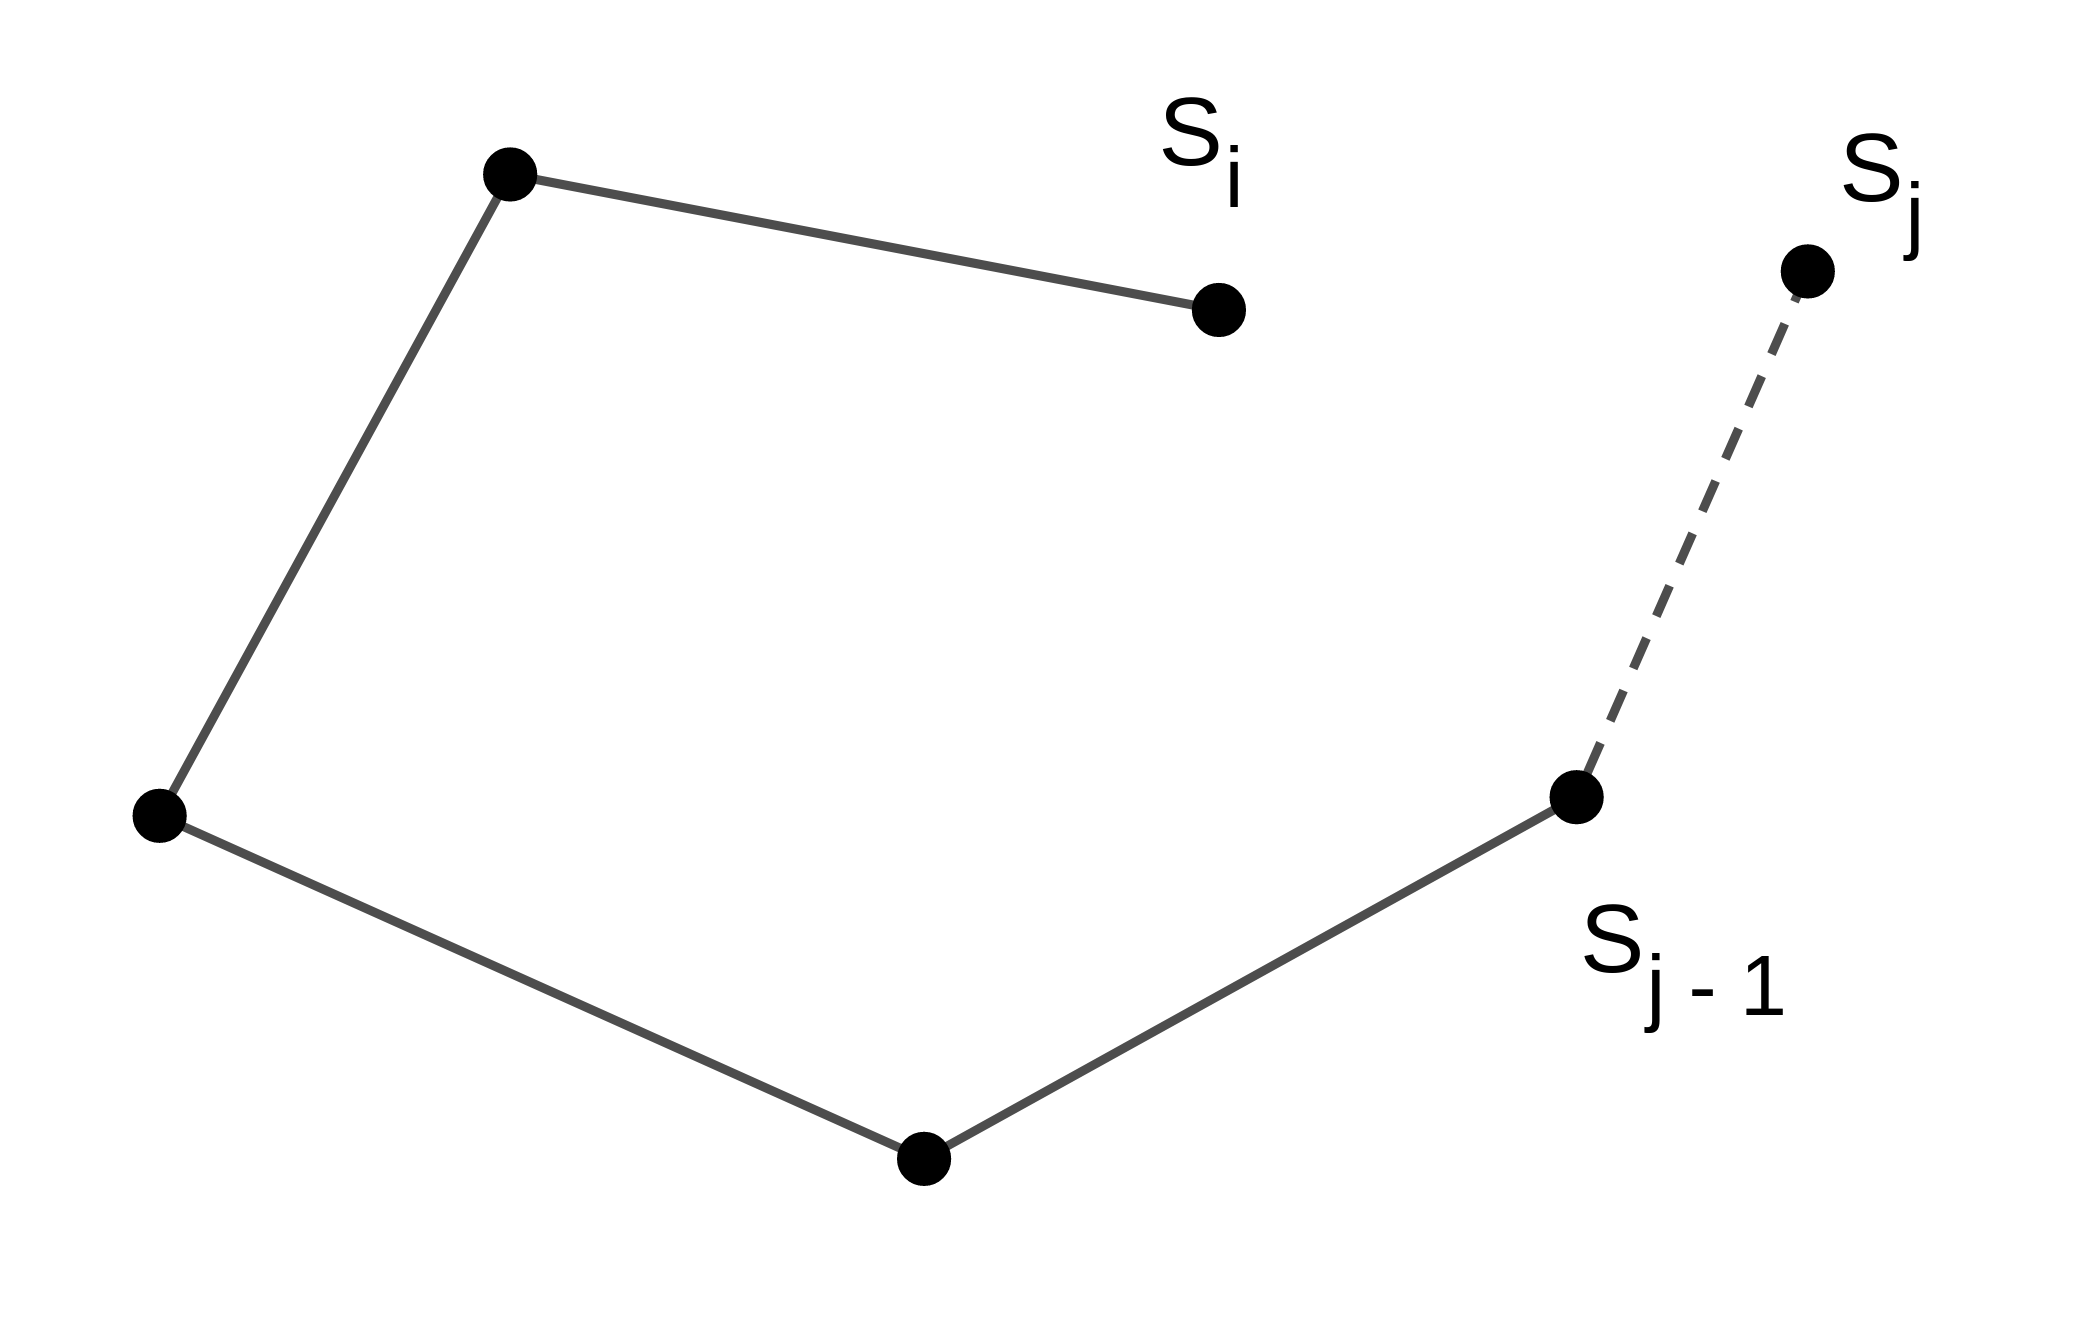
\includegraphics[scale=0.20]{1.png}
        \hspace{1cm}
        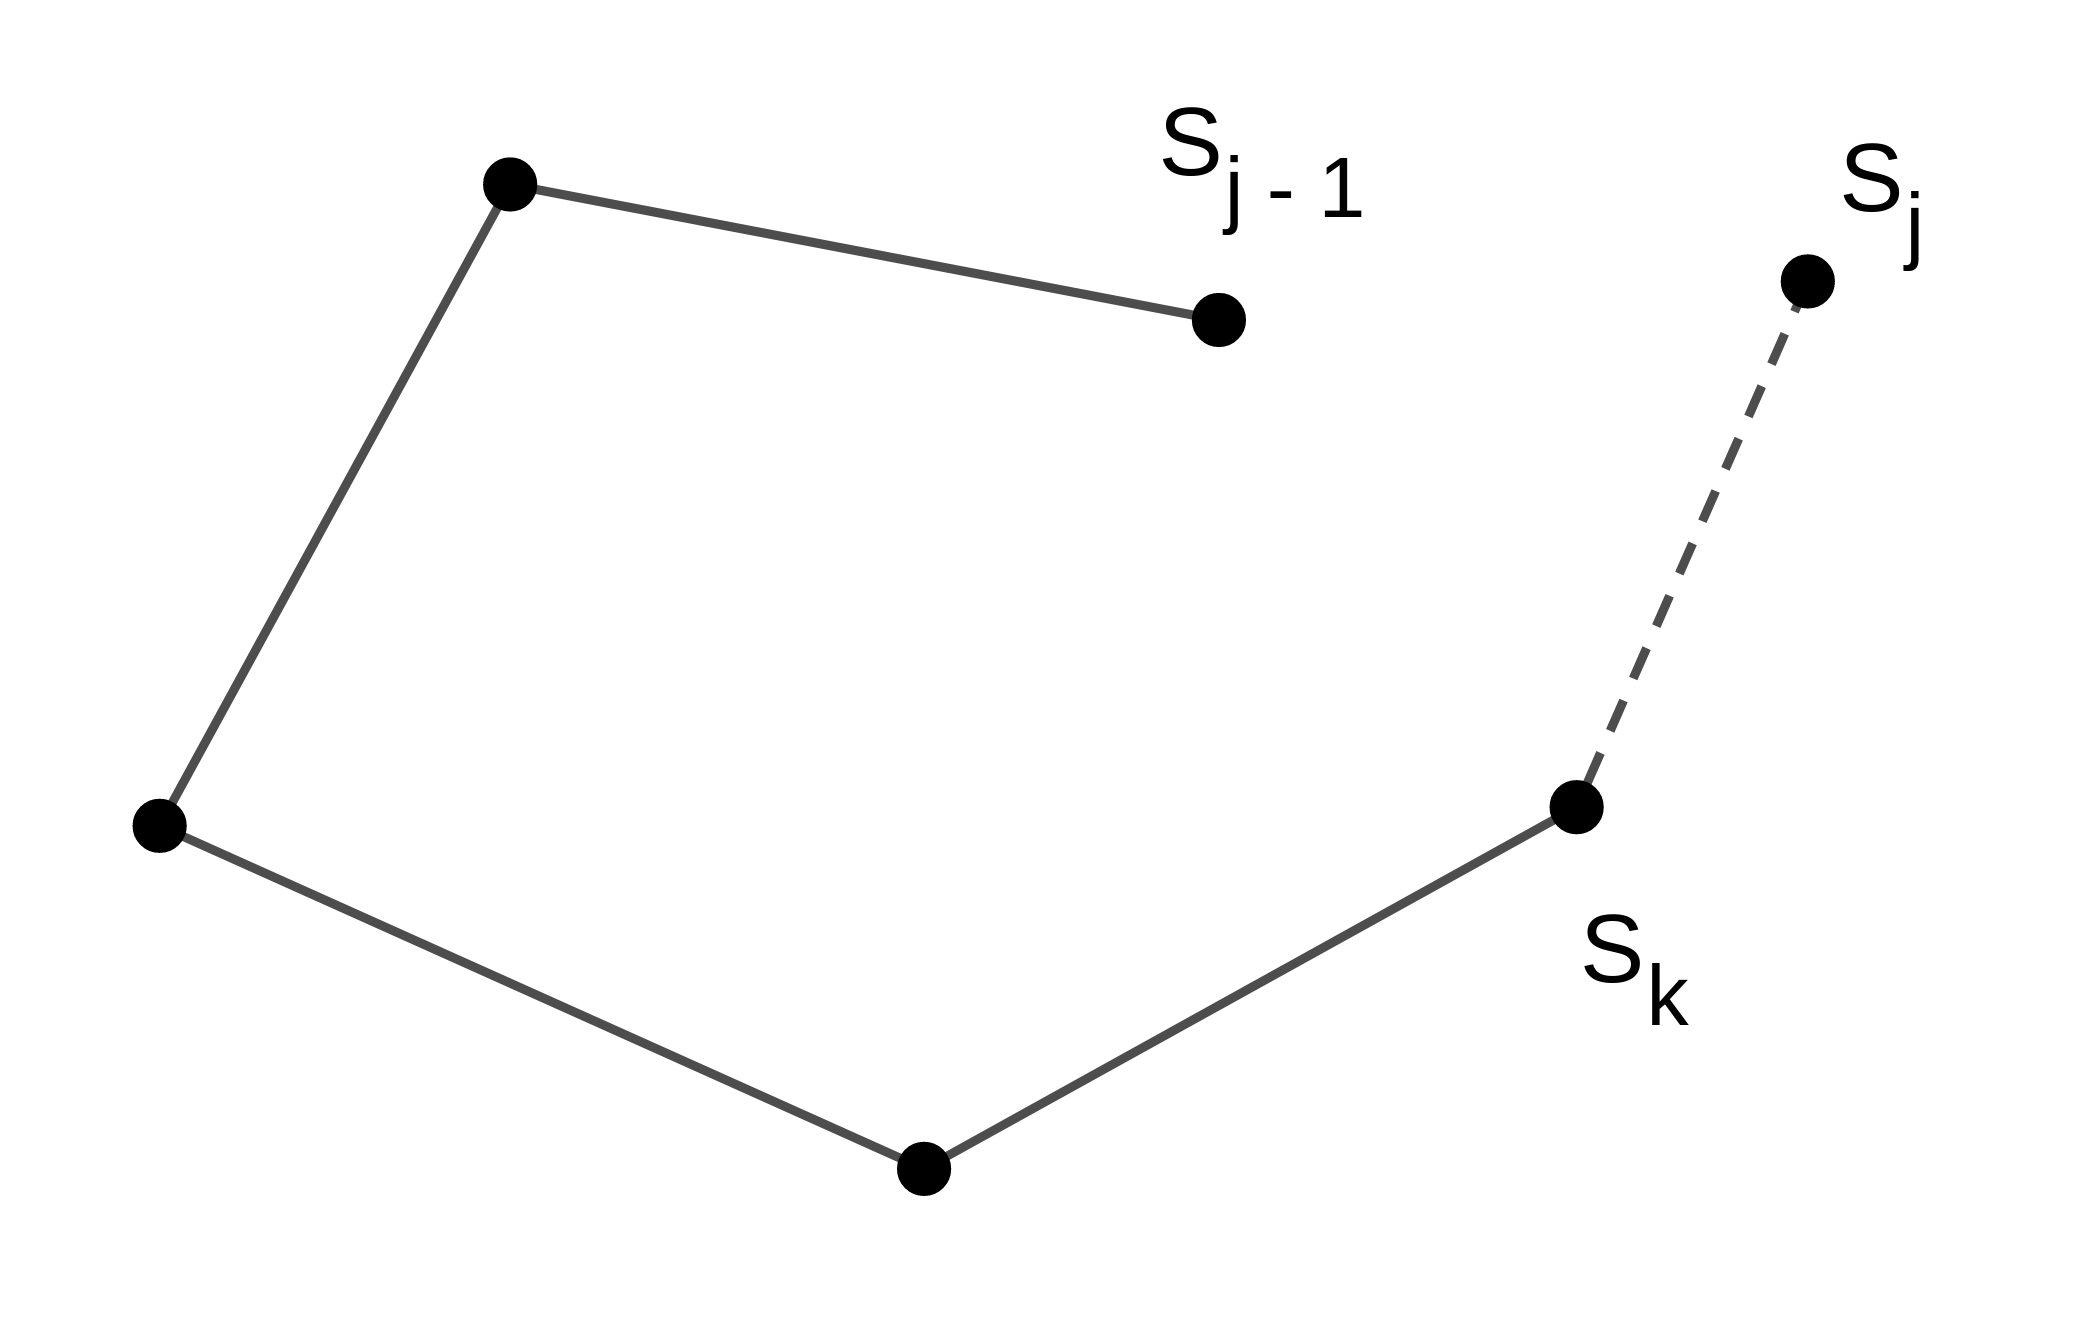
\includegraphics[scale=0.20]{2.png}
        \caption{Cases $1$ and $2$}
        \label{fig:poly1}
    \end{figure}

    Let's define $M[1..n][1..n]$, where $M[i][j]$ stores the minimal value of $p(Q_{ij})$ 
    with $S_i$ and $S_j$ as terminal vertices of the vertex chains. 
    Now the recurrence relation for the DP, such that $S_j$ is the vertex to be added and 
    $\forall\,i,\,j\,\epsilon\,\{1,..,n\},\,i\le\,j$, can be defined as:
    
    \begin{equation}
        M[i][j]=
        \begin{cases}
            M[i][j-1]\,+\,dist(j-1,\,j), & \text{$i\,\textless\,j-1$}\\
            \min\limits_{1\,\le\,k\,\textless\,j}\{M[i][k]\,+\,dist(k,\,j)\}, & 
            \text{$i\,=j-1$ or $i\,=\,j$}\\
            -1, & \textit{else}\\
        \end{cases}\\
    \end{equation}

    So, the perimeter of the optimal polygon $Q$ will be, $p(Q_{nn})\,=\,M[n][n]$.
    
  \section{Algorithm}
    
    Now that Optimal Substructure has been defined, let's design the algorithm. Before 
    that, we can see there are \textbf{overlapping sub-problems} (e.g. $M[3][1]$ will
    be required for $M[3][3]$). So, \textbf{memoization} will be used.
    
    To solve the problem, we store the minimal value of the perimeter $p(Q_{ij})$, 
    $\forall\,S_i,\,S_j\,\epsilon\,\{S_1,..,S_n\}$ using equation $(1)$. For this we 
    construct a matrix $M[0..n][0..n]$, where $M[i][j]$ stores the minimal value of 
    the perimeter $p(Q)$ of the polygon $Q_{ij}$ with $S_i$ and $S_j$ as terminal vertices
    of the vertex chains. To store the polygon $Q$, we construct a $T[0..n][0..n]$, where
    $T[i][j]$ stores the pair of terminal vertices of the open chains just before adding 
    $S_j$ vertex. Bottom-up approach will be used to fill matrix $M$.\\
    
    \newline\newline \textbf{Main Steps:}
    \begin{enumerate}
        \item Sort the point set $P$ in increasing $x$-coordinate and store in list $S$.
        \item Initialize the matrix $M$ with $-1$ values. $M[i][j]=-1$ denotes that open 
        polygon $Q_{ij}$ with $S_i$ and $S_j$ as terminal vertices of the vertex chains is
        not to be considered. Set $M[1][1]\,=\,0$, as the base case.
        \item Consider any open polygon $Q_{ij}$ and calculate the minimum perimeter 
        $p(Q_{ij})$ using equation $(1)$. Accordingly, update $T[i][j]$.
        \item $M[n][n]$ is the minimum perimeter $p(Q_{nn})$ for the polygon $Q$.
        \item To get the polygon $Q$, we trace back from $T[n][n]$ up to $T[1][1]$ and 
        store the two chains.
    \end{enumerate}
    
  \section{Time and space complexities}
  
    \subsection{Time Complexity}
    Let's refer to the above mentioned steps for calculation of time complexity.
    \begin{enumerate}
        \item Sorting $n$ points $\rightarrow\,O(n\log(n))$ time.
        \item In equation $(1)$, the $1^_{st}$ condition takes $O(n^2)$ time and the 
        $2^_{nd}$ condition takes $O(n)$ time. So, for Step $3$ $\rightarrow\,O(n^2)$
        time.
    \end{enumerate}
    So, overall Time complexity $=\,O(n^2)$.
    
    \subsection{Space Complexity}
    As a matrix $M[0..n][0..n]$ is constructed, the space complexity of the algorithm 
    will also be $O(n^2)$.\\
    
\end{document}
